\documentclass{beamer}

% Packages

% Sets

% Formal statements


\title{Diseño y análisis de algoritmos \\ ISIS1105}
\author{Daniel R. Barrero R.}
\institute{Universidad de los Andes}

\begin{document}
\frame{\titlepage}

%

\begin{frame}{Big-O notation}
	Let $f : \NN \to \Rpos$. We define

	\begin{equation*}
		O(f) = \{\tau : \NN \to \Rpos | \exists C \in \Rpos, N \in \NN:
		\ \forall n \geq N:\ \tau(n) \leq Cf(n)\}
	\end{equation*}

	\textbf{True or false?}
	\begin{itemize}
		\item $10n^2 \in O(n^3)$
		\item $10n^2 \in O(n^2)$
		\item $n^3 \in O(10n^2)$
		\item $n|\sin(n\pi/2)| \in O(n)$
		\item $n \in O(n^2|\sin(n\pi/2)|)$
	\end{itemize}
\end{frame}

%

\begin{frame}{Recursive algorithms and recurrence relations}
	Consider the recursive way to compute Fibonacci numbers:

	\lstinputlisting[language=Java, firstline=23, lastline=28]{Aula03.java}

	If we overlook the cost of addition, and let $t(n)$ denote the execution
	time of algorithm \texttt{fibRec} for input $n \in \NN$, we may assume that
	$t(n)$ satisfies the initial value problem
	\begin{displaymath}
		\begin{cases}
			t(0)= 1,\ t(1)= 1 \\
			t(n)= t(n-1) + t(n-2),\ n \geq 2
		\end{cases}
	\end{displaymath}
\end{frame}

%

\begin{frame}{Linear homogeneous recurrence relations}
	Can we find a \emph{closed formula} for $t(n)$?

	\bigskip
	Namely, can we solve
	\begin{displaymath}
		\begin{cases}
			t(0)= 1,\ t(1)= 1 \\
			t(n)= t(n-1) + t(n-2),\ n \geq 2
		\end{cases}
	\end{displaymath}

	so that the value $t(n)$ depends only on $n$ and not on previous values
	of $t$?
\end{frame}

%

\begin{frame}{Linear homogeneous recurrence relations (LHRRs)}
	Consider the sequence of powers $(a_n)_{n=0}^\infty$ given by $a_n = (-3)^n$.

	\bigskip
	Namely,
	\begin{equation*}
		(a_n)_{n=0}^\infty = 1, -3, 9, -27, \cdots
	\end{equation*}

	It is a solution of 
	\begin{displaymath}
		t(n)= -3t(n-1),
	\end{displaymath} 

	but not of
	\begin{displaymath}
		t(n)= 2t(n-1).
	\end{displaymath}

	Notice that $(-3)^n$ is also a solution of
	\begin{displaymath}
		t(n)= -t(n-1) + 6t(n-2).
	\end{displaymath}
\end{frame}

%

\begin{frame}{LHRRs}
	\begin{defn}
		Consider the relation
		\begin{equation}\label{lhrr}
			t(n)= a_1t(n-1) + \cdots + a_{k-1}t(n-k+1) + a_kt(n-k).
		\end{equation}
		We call it a \emph{linear homogeneous recurrence relation (lhrr)}.
		The \emph{characteristic equation} of \eqref{lhrr} is
		\begin{equation}\label{cheq}
			x^k - a_1x^{k-1} - \cdots - a_{k-1}x - a_k = 0,
		\end{equation}
		its solutions are called the \emph{roots} of \eqref{lhrr}, and $k$ is
		the \emph{degree} of \eqref{lhrr}.
	\end{defn}
\end{frame}

%

\begin{frame}{Quiz}
		For the Fibonacci relation
		\begin{equation*}
			t(n)= t(n-1) + t(n-2)
		\end{equation*}
		\begin{itemize}
			\item Determine its degree
			\item Write down its characteristic equation
			\item Compute its roots
		\end{itemize}
\end{frame}

%

\begin{frame}{LHRRs}
	\begin{thm}[1]\label{thmhr}
		The initial value problem
		\begin{displaymath}
			\begin{cases}
				t(0)= v_0,\ t(1)= v_1,\cdots t(k-1)= v_{k-1}\\
				t(n)= a_1t(n-1) + \cdots + a_{k-1}t(n-k+1) + a_kt(n-k)
			\end{cases}
		\end{displaymath}
		has a unique solution
		\begin{equation*}
			t(n) = c_0\alpha_0^n + c_1\alpha_1^n + \cdots + c_{k-1}\alpha_{k-1}^n
		\end{equation*}
		where the $c_i$ are complex numbers and the $\alpha_i$ are the roots of
		the lhrr.
	\end{thm}
\end{frame}

\begin{frame}{LHRRs}
	\textbf{Exercise}. Solve the initial value problem of the \texttt{fibRec}
	algorithm.
	\begin{displaymath}
		\begin{cases}
			t(0)= 1,\ t(1)= 1\\
			t(n)= t(n-1) + t(n-2)
		\end{cases}
	\end{displaymath}
\end{frame}

%% Final lhrr slide - exercises
\begin{frame}{LHRRs - exercises}
	\textbf{Exercise}. Solve the recurrence
	\begin{displaymath}
		\begin{cases}
			t(0)= 4\\
			t(n)= 3t(n-1).
		\end{cases}
	\end{displaymath}
	%
	\textbf{Exercise}. Solve the recurrence
	\begin{displaymath}
		\begin{cases}
			t(0)= 1,\ t(1)= 2\\
			t(n)= -t(n-1) + 6t(n-2)
		\end{cases}
	\end{displaymath}
	%
	\textbf{Exercise}. Find the recurrence of which $\sqrt{3}(-3)^n - \sqrt{2}2^n$
	is the solution.
\end{frame}

%

%% Inhomogeneous linear
\begin{frame}{The towers of Hanoi}
	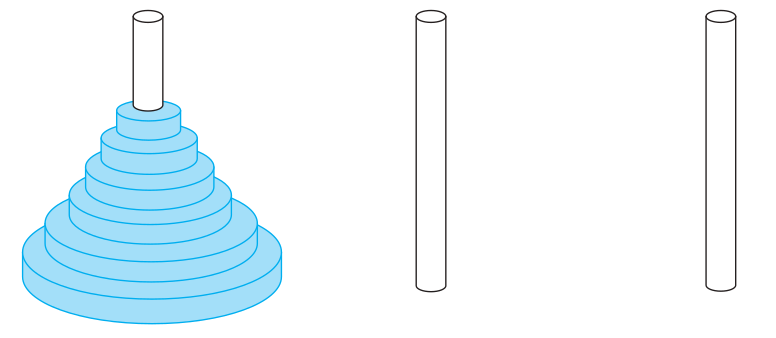
\includegraphics[width=0.5\textwidth]{hanoi.png}

	\begin{itemize}
		\item[]
		\item Poner los discos en orden de tamaño en la segunda clavija,
			moviendo un disco a la vez.
		\item No se puede poner un disco más grande sobre uno más pequeño.
	\end{itemize}
\end{frame}

%

\begin{frame}{The towers of Hanoi}
	\lstinputlisting[language=Java, firstline=2, lastline=17]{Aula04.java}
\end{frame}

%

\begin{frame}{LRRs - The towers of Hanoi}
	The associated initial value problem is
	\begin{displaymath}
		\begin{cases}
			t(0)= 0\\
			t(m)= 2t(m-1) + 1,\ m \geq 1.
		\end{cases}
	\end{displaymath}
	and its recurrence relation is \emph{not} homogeneous.
	\begin{defn}
		A \emph{linear recurrence relation (lrr)} is of the form
		\begin{equation}\label{lrr}
			t(n) + b_1t(n-1) + \cdots + b_{k-1}t(n-k+1) + b_kt(n-k)= q.
		\end{equation}
		When $q \neq 0$, it is called the \emph{inhomogeneous part} of \eqref{lrr}.
	\end{defn}
\end{frame}

%

\begin{frame}{LRRs - The towers of Hanoi}
	If $t(n) - 2t(n-1) = 1$ for all $n \geq 1$, then $t(n-1) - 2t(n-2) = 1$ for
	all $n \geq 2$. Therefore, the Hanoi problem can be reformulated as

	\begin{displaymath}
		\begin{cases}
			t(0)= 0,\ t(1)= 1\\
			t(n)= 3t(n-1) - 2t(n-2),\ n \geq 2.
		\end{cases}
	\end{displaymath}
	Thanks to theorem \ref{thmhr}, its solution is of the form
	\begin{equation*}
		t(n) = c_02^n + c_11^n,
	\end{equation*}
	where the constants $c_0$ and $c_1$ can be found by solving the linear
	system
	\begin{displaymath}
		\begin{cases}
			c_0 + c_1 = 0\\
			2c_0 + c_1 = 1.
		\end{cases}
	\end{displaymath}
\end{frame}

%

\begin{frame}{LRRs - reduction to homogeneous case}
	We solved the inhomogeneous Hanoi problem by making it a particular case
	of a higher-degree homogeneous problem. This applies in general for the
	following family of problems.
	\begin{thm}[2]
		If the initial value problem
		\begin{displaymath}(4)
			\begin{cases}
				t(0)= v_0, \cdots, t(k-1)= v_{k-1}\\
				\sum_{i= 0}^k b_it(n-i)= q,\ n \geq k
			\end{cases}
		\end{displaymath}
		is such that $q = c^np(n)$, where $c$ is a positive constant and
		$p(n)$ is a polynomial of degree $d$, then it is equivalent to a
		homogeneous problem of degree $k+d+1$ with characteristic equation
		\begin{equation*}
			E(x)(x-c)^{d+1} = 0
		\end{equation*}
		where $E(x) = 0$ is the characteristic equation of (4).
	\end{thm}
\end{frame}

%% Divide and conquer
\begin{frame}{Divide and conquer}
	Consider the merge sorting algorithm
	\lstinputlisting[language=Java, firstline=28, lastline=49]{Aula04.java}
\end{frame}

%

\begin{frame}{Divide and conquer}
	Its time complexity satisfies the initial value problem
	\begin{displaymath}
		\begin{cases}
			t(1)= 1\\
			t(n)= t\left( \lceil n/2 \rceil \right) +
			t\left( \lfloor n/2 \rfloor \right) + n,\ n \geq 2.
		\end{cases}
	\end{displaymath}
\end{frame}
\end{document}
